%%%%%%%%%%%%%%%%%%%%%%%%%%%%%%%%%%%%%%%%%%%%%%%%%%%%%%%%%%%%%%%%%%%%%%%%%%%%%%%%
%Objetivo: Propor um conjunto de recomendações de melhorias para as
% 		   as funcionalidade das FGRMs
%Autores: Vagner Clementino <vagnercs@dcc.ufmg.br>
%		  Rodolfo Resende <rodolfo@dcc.ufmg.br>
%Criação: dom fev 26 12:49:27 BRT 2017
%Modificação:: sáb mai 13 14:17:28 -03 2017
%Revisão: dom abr 23 23:16:51 -03 2017
%%%%%%%%%%%%%%%%%%%%%%%%%%%%%%%%%%%%%%%%%%%%%%%%%%%%%%%%%%%%%%%%%%%%%%%%%%%%%%%%
\chapter{Sugestões de Melhorias para as FGRMs}
\label{ch:sug_melhoria}

\section{Introdução}
\label{sec:sug_melhoria_intro}

No levantamento por questionário descrito no
Capítulo~\ref{ch:pesquisa-profissionais} os profissionais consultados se
mostraram, em geral, satisfeitos com as funcionalidades disponibilizadas pelas
FGRMs. Cerca de 90\% dos par\-ti\-ci\-pan\-tes fizeram uma avaliação positiva da
ferramenta que utilizam, além disso, também cerca de 90\% dos participantes
disseram que recomendariam as FGRMs que utilizam para um novo projeto.

Não obstante, naquela mesma pesquisa, apresentamos uma lista de possíveis novas
funcionalidades para as FGRMs e perguntamos ao participante quais
funcionalidades ele desejaria que fosse incluída  em sua FGRM\@. O resultado
desta pergunta foi que cerca de 85\% se mostraram interessados na inclusão de
pelo menos uma das funções propostas na FGRM que utiliza. A partir da análise
deste resultado é possível inferir que os desenvolvedores estão satisfeitos com
a ferramenta utilizada, contudo, \textit{não conhecem ou não têm acesso ao
    potencial de funcionalidades que este tipo de software pode oferecer}.

Diante do exposto, entendemos que podemos contribuir com o estado a\-tu\-al das
funcionalidades das FGRMs propondo um conjunto de melhorias. As sugestões foram
compiladas utilizando a literatura da área e os levantamentos realizados nesta
dissertação, especialmente com base nos
Capítulos~\ref{ch:mapeamento-sistematico} e~\ref{ch:pesquisa-profissionais}, na
Seção~\ref{sec:caracterizacao_ferramentas} e nos estudos que propõem melhorias
para as FGRM~\cite{zimmermann2009improving, bettenburg2008makes, singh2011bug}.
Estas recomendações podem ser utilizadas por pesquisadores interessados em
conduzir estudos sobre o avanço da produtividade dos desenvolvedores mediante o
uso das FGRMs. Além disso, os responsáveis pelo desenvolvimento deste tipo de
software, podem utilizar algumas das recomendações para a criação ou
aperfeiçoamento das funcionalidades da FGRM que é responsável. Na mesma linha,
os profissionais envolvidos com Manutenção de Software podem criar extensões
(plugins) com base no que foi proposto de modo a aplicar essas melhorias em sua
rotina de trabalho.

Este capítulo está organizado da seguinte forma: a
Seção~\ref{sec:sug_melhoria_melhorando_as_ferraementas} apresenta as sugestões
de melhorias propostas, cada sugestão é seguida de uma breve discussão de como
foi obtida e justificativa de sua consideração; na
Seção~\ref{sec:sug_melhoria_avaliacao_das_melhorias} realizamos uma avaliação do
que foi recomendado com base na opinião de profissionais que contribuem para
projetos relacionados ao desenvolvimento de FGRMs; os resultados do processo de
avaliação são apresentados na
Seção~\ref{sec:resultados_avaliacao_sug_de_melhorias}; na
Seção~\ref{sec:sug_melhoria_discussao} discutimos os resultados obtidos no
processo de avaliação; na Seção~\ref{sec:sug_melhoria_ameacas} apresentamos as
ameaças à validade; encerramos o capítulo com um resumo na
Seção~\ref{sec:sug_melhoria_resumo}.

\section{Sugestões de Melhorias para FGRMs}
\label{sec:sug_melhoria_melhorando_as_ferraementas}

As sugestões propostas neste capítulo não estão vinculadas exclusivamente à
melhorias de funcionalidades existentes nas FGRMs. As recomendações podem
representar o desenvolvimento de um novo comportamento ou a melhoria de outros
já existentes. Cabe-nos ressaltar que o conjunto proposto não é exaustivo e é
baseado nos resultados desta dissertação.

É possível que algumas das recomendações propostas já estejam implementadas de
maneira parcial ou integral.  Infelizmente não tivemos como verificar isso em
função do esforço exigido pelo grande volume de ferramentas disponíveis quando
esta dissertação foi escrita. Além disso, o processo de validação descrito na
Seção~\ref{sec:sug_melhoria_avaliacao_das_melhorias} pôde nos alertar sobre a
eventual proposição de uma funcionalidade existente. Ao longo da elaboração das
sugestões verificamos que não conseguiríamos implementá-las e também não
conseguiríamos analisar a complexidade de estratégias de implementação.
Entretanto, como prova de conceito, a sugestão descrita na
Seção~\ref{sub:supote_a_qualidade_do_relato} foi implementada como extensão de
do repositório de RMs da plataforma Github, conforme pode ser visto no
Capítulo~\ref{ch:implemtacao_extensao}. As sugestões realizadas foram
estruturadas como seções deste capítulo, em que apresentamos a
\textit{justificativa, o benefício gerado, as limitações e exemplos de
    utilização.}

\subsection{Suporte à Qualidade do Texto Relatado}
\label{sub:supote_a_qualidade_do_relato}

\sugestao{01}{As FGRMs devem fornecer realimentação (feedback) relacionado com a
    qualidade do texto relatado.}

\paragraph{Justificativa:}
\label{par:justificativa_s01}

Conforme discutido na
Seção~\ref{subsec:man_visao_geral_papeis_na_manutencao_de_software} o
responsável por reportar uma RM pode ser tanto um usuário do sistema quanto um
membro da equipe de desenvolvimento ou manutenção. Por esta razão, podemos
encontrar Reportadores com diferentes níveis de conhecimento sobre o sistema.
Do ponto de vista dos desenvolvedores, um problema recorrente é a baixa
qualidade do texto no relato da RM, tipicamente a falta da informação necessária
à solução. Alguns estudos mostram que a ausência das etapas para reproduzir a
falha e a ausência da cadeia de registros de ativação dificultam mais o
andamento do projeto do que a ocorrência de RMs
duplicadas~\cite{bettenburg2008makes, bettenburg2007quality}. Neste sentido, as
FGRMs poderiam fornecer uma funcionalidade capaz de reduzir o número de relatos
de baixa qualidade através, por exemplo, de uma realimentação ao Reportador
envolvendo uma estimativa da qualidade do que foi informado no relato da RM\@.

\paragraph{Benefício Gerado:}
\label{par:beneficio_s01}

Com este tipo de funcionalidade uma FGRM poderia reduzir o tempo de análise das
RMs pelo fato que o responsável por criá-la estaria ciente das informações
necessárias à sua solução. Neste caso, o desenvolvedor seria diretamente
beneficiado já que teria a sua disposição um relato mais completo. Não obstante,
um trabalho adicional seria dado aos reportadores que em algumas situações devem
rever as informações incluídas na RM\@.

\paragraph{Limitações:}
\label{par:limitacoes_s01}

Alguns estudos sobre a melhoria da qualidade do relato da RM focam
prioritariamente nas requisições que descrevem defeitos do software. Conforme
discutimos na Seção~\ref{sec:requisicao_de_mudanca}, uma RM pode também estar
relacionada com um pedido de melhoria. Uma dificuldade desta recomendação de
funcionalidade é separar de forma automatizada as duas dimensões das RMs. Da
mesma forma, seria importante definir padrões distintos para analisar a
qualidade do relato por conta de suas diferentes características e necessidades
de uma RM\@.

\paragraph{Exemplo de Utilização:}
\label{par:exemplo_s01}

Após o usuário relatar um problema ou pedido de melhoria, a ferramenta de
poderia avaliar o texto corresponde ao atributo \textit{relato} da RM gerada e
apresentar ao responsável realimentação sobre como a informação fornecida
poderia ser melhorada, como por exemplo através da inclusão de um arquivo com o
histórico de execução do software (log). Como prova de conceito foi implementada
uma extensão para uma FGRM com estas características no
Capítulo~\ref{ch:implemtacao_extensao}.

\subsection{Acesso Facilitado ao Código Fonte Incluído nas RMs}
\label{sub:busca_por_código_fonte}

\sugestao{02}{As FGRMs deveriam fornecer busca pelo código fonte contido no
    relato, comentários ou anexos das RMs.}

\paragraph{Justificativa:}
\label{par:justificativa_s02}

As RMs permitem a inclusão de fragmentos de código fonte em seu relato ou nos
comentários em diversas etapas do seu ciclo de vida. O código pode ser incluído
durante a criação das RMs, nas discussões realizadas para a sua solução ou mesmo
quando ela é concluída (fechada). Quando o código corresponde a uma solução
então recebe o nome de \textit{patch}. Os fragmentos de código podem ser
utilizados para descrever uma falha ou apresentar uma solução candidata. Apesar
de sua importância este tipo de informação não é facilmente recuperada no
contexto de uso de uma FGRM\@. O estudo de Damevski e
outros~\cite{damevski2016field}, que analisa o problema da localização de
funcionalidades no código fonte (feature location), ressalta a importância da
facilidade de acesso ao código fonte pode propiciar a redução do tempo de
conclusão da tarefa de manutenção e o aumento da qualidade das alterações
realizadas. Este é um caso particular de uma sugestão de melhoria que envolve
generalizar ou especializar a interface de busca das FGRMs. Esta interface tem
relação com a sugestão \#06 porque pode ser só texto (Recuperação da Informação)
ou pode envolver elementos não textuais.

\paragraph{Benefício Gerado:}
\label{par:beneficios_s02}

Com um fácil acesso ao código fonte um desenvolvedor pode obter exemplos de
solução para RMs similares. Este tipo de funcionalidade pode ser vantajosa em
comparação com a busca estruturada, presente em grande parte das FGRMs, por
permitir a recuperação com base em elementos específicos da linguagem de
programação utilizada pelo software que a FGRM suporta, como por exemplo
classes, funções, constantes e outros.

\paragraph{Exemplo de Utilização:}
\label{par:exemplo_s02}

Em certas ocasiões, uma RM em análise pode ter similaridades com outras
solucionadas anteriormente. A similaridade pode ser devido a afetarem o mesmo
módulo do sistema, por exemplo. Um desenvolvedor poderia realizar uma busca por
código fonte na RM solucionada com o objetivo de encontrar fragmentos de código
que o ajudem no entendimento e solução do pedido atual.

\subsection{Ranqueamento pela Reputação do Reportador}
\label{sub:diferenciacao_do_reportdor}

\sugestao{03}{As FGRMs deveriam permitir um ranqueamento das RMs de acordo com a
reputação do Reportador.}

\paragraph{Justificativa:}
\label{par:justificativa_s03}

Um problema recorrente em diversos projetos de software é a definição da ordem
que o conjunto de RMs deve ser analisado. Conforme discutido na
Seção~\ref{ssub:melhorias_dim_processo} alguns estudos vêm se dedicando em
classificar as RMs sob determinados critérios. Por outro lado, é possível
observar que determinados \textit{Reportadores} têm por hábito relatar pedidos
que possuem um maior grau de relevância no projeto. Por exemplo, existem certos
usuários que geralmente relatam RMs relativas à questões de segurança do
sistema. Neste contexto, seria interessante se as FGRMs aplicassem algum tipo de
métrica de relevância aos seus usuários, em especial aos reportadores. Em um
segundo momento, esta mesma medida poderia ser utilizada com a finalidade de
ranquear as RMs. Neste sentido, conforme a conveniência, um desenvolvedor
poderia priorizar as requisições de reportadores com um maior grau de reputação.

%Sejam relevantes ao projeto de software, tais requisições deveriam receber algum
%tipo de etiqueta de modo a diferenciá-las dentro da FGRM\@. Segundo o nosso
%entendimento uma RM pode ser classificada como relevante se descreve um problema
%que afeta um grande número de usuários do sistema ou representa uma falha de
%segurança do software. Além disso deve ser redigida de forma clara e fornecer as
%informações necessárias para sua solução. O grau de relevância de determinada RM
%pode variar em diferentes projetos e pode depender de critérios subjetivos de
%quem analisa.

\paragraph{Benefício Gerado:}
\label{par:papéis_afetados_s03}

Uma das possíveis atividades desempenhadas pelo \textit{Agente de Triagem} é
definir o desenvolvedor mais apto para determinada RM\@. Ele pode utilizar
diversos critérios no exercício desta atividade, como por exemplo a prioridade
do que foi relatado. Segundo a nossa proposta, o \textit{Agente de Triagem} pode
previamente ordenar uma lista de RMs pelo grau de reputação de quem as redigiu.
A partir disso, ele poderia atribuir primeiro as RMs de Reportadores com maior
grau de reputação. Com base nesta estratégia, é possível que RMs com maior
relevância sejam analisadas primeiro. O conceito de relevância pode variar em
diferentes projetos. Contudo, uma RM poderia ser classificada como relevante
caso descreva um problema que afete um grande número de usuários ou represente
uma falha de segurança do software. Além disso, deve ser redigida de forma clara
e fornecer as informações necessárias para sua solução.

\paragraph{Exemplo de Utilização:}
\label{par:exemplo_de_utilização_s03}

Conforme descrito anteriormente, um \textit{Agente de Triagem} poderia ordenar
uma lista de RMs pelo grau de reputação do \textit{Reportador}. Em seguida daria
início ao processo de atribuição analisando primeiro as RMs mais bem ranqueadas.
Caso as elas sejam relevantes o profissional poderia realizar a atribuição.

\subsection{Atalhos para filtros e classificação (rankings) das RMs}
\label{sub:histórico_das_ùltimas_rm_s}

\sugestao{04}{As FGRMs deveriam fornecer atalhos para filtros
    per\-so\-na\-li\-zá\-veis e classificações (rankings).}

\paragraph{Justificativa:}
\label{par:justificativa_s04}

As RMs atribuídas a determinado desenvolvedor podem estar em diferentes estados.
Existem aquelas que não foram analisadas, que estão aguardando informações
adicionais ou que estejam aguardando o Analista de Qualidade, por exemplo. Em
geral, conforme discutido na Seção~\ref{sec:caracterizacao_ferramentas}, as
FGRMs permitem visualizar a situação das RMs de um desenvolvedor mediante
relatórios pré-definidos. Contudo, no levantamento mediante questionário,
apresentado no Capítulo~\ref{ch:pesquisa-profissionais}, identificamos que uma
parte dos profissionais solicitou um acesso mais facilitado a este tipo de
informação. Desta forma, sugerimos uma alteração nas interfaces das FGRMs de
modo a fornecer acesso facilitado a filtros personalizáveis e outros tipos de
classificações.

\begin{itemize}
	\item Conforme relato dos participantes eles gostariam:
	\begin{itemize}
		\item \textit{``The ability to clearly visualize how many tickets are at
				the to do, in progress, to validate or done steps.''}.
		\item \textit{``History tracking, commenting, attachments, priority
				setting, task assignment, tie in with deployment systems.''}
	\end{itemize}
\end{itemize}

\paragraph{Benefício Gerado:}
\label{par:papéis_afetados_s04}

Com um acesso mais rápido às últimas RMs analisadas o desenvolvedor poderia ter
uma noção geral do trabalho desenvolvido. Este panorama poderia ajudá-lo no
planejamento de suas atividades diárias.

\paragraph{Exemplo de Utilização:}
\label{par:exemplo_de_utilização_s04}

Ao acessar a FGRM o desenvolvedor tem acesso as últimas $n$ RMs que ele
analisou. Além disso, ele poderia criar filtros para acessar outras informações
que julgar importante no desenvolvimento de suas atividades.

\subsection{Suporte à Processos de Integração Contínua}
\label{sub:suporte_integracao_continua}

\sugestao{05}{As FGRMs deveriam fornecer suporte à Processos de Integração
    Contínua.}

\paragraph{Justificativa:}
\label{par:justificativa_s05}

A solução de determinada RM pode levar a resultados não esperados em outros
módulos do sistema mantido. Para tomar conhecimento dos possíveis problemas
recomenda-se a avaliação do impacto da RM\@. A Análise de Impacto estima o que
será afetado no software e na documentação relacionada caso uma mudança proposta
seja feita~\cite{arnold1996software}. A literatura sobre RMs discute algumas
soluções com o objetivo de realizar a Análise de Impacto. Alguns exemplos de
trabalhos nesta linha são apresentados na
Seção~\ref{ssub:melhorias_dim_processo}. Dentro das propostas feitas pelos
agilistas uma das possibilidades de reduzir os efeitos colaterais de uma mudança
é periodicamente realizar a construção (build) do sistema. A \textit{Integração
    Contínua} (IC) é a prática de construir e implantar (deploy) imediatamente
após um desenvolvedor compromissar (commit) o código
fonte~\cite{aiello2010configuration}. Neste sentido, as FGRMs poderiam vincular
a solução de uma RM com a execução do processo de IC\@. Desta forma, seria
possível associar uma versão do sistema com o conjunto de RMs solucionadas até a
sua geração. Este tipo de integração foi descrita como uma funcionalidade
ausente nas FGRMs por alguns participantes do levantamento por questionário
descrito no Capítulo~\ref{ch:pesquisa-profissionais}.

\paragraph{Benefício Gerado:}
\label{par:papéis_afetados_s05}

A integração de uma FGRM com processos de IC traria para as atividades de
manutenção os benefícios desta prática, tais como a redução de riscos e a
facilidade de encontrar e remover falhas~\cite{fowler2006continuous}.  Além
disso, segundo o nosso entendimento, o fato de associar a solução de uma RM com
determinada versão de um sistema, pode minimizar problemas levantados no
Mapeamento Sistemático descrito no Capítulo~\ref{ch:mapeamento-sistematico}, por
exemplo a Localização do Problema (Seção~\ref{ssub:melhorias_dim_ferramenta}) e
a Estimativa de Esforço da RM (Seção~\ref{ssub:melhorias_dim_processo}). Em
ambos os casos é possível aproveitar a facilidade que a IC propicia em fornecer
a localização de uma falha que, por exemplo, pode ter sido causada pela solução
de uma RM\@.

\paragraph{Limitações:}
\label{par:limitacoes_s05}

Algumas vezes a mudança de situação de uma RM para \textit{Fechada} pode não
representar a sua efetiva solução. Por exemplo, a falha descrita pode ser
definida como de baixo impacto e desta maneira não ser tratada, ou ainda o
conjunto de fatores que geraram o problema descrito na RM deixa de existir.
Nestas situação não faz sentido que responsável por fechar a RM engatilhe um
processo de Integração Contínua.

\paragraph{Exemplo de Utilização:}
\label{par:exemplo_de_utilização_s05}

Após um desenvolvedor solucionar determinada RM, mudando a sua situação para
\textit{Fechada}, por exemplo, a FGRM dispara o processo de compilação do
sistema. O resultado da compilação poderia ser exibido em um painel de controle
incluindo o responsável pela mudança mais recente no sistema e as compilações
que resultaram em falhas. O painel poderia incluir ainda dados da RM que
engatilhou o processo de compilação como por exemplo o seu número e título.

\subsection{Suporte além do Texto Simples}
\label{sub:suporte_linguagem_marcacao}

\sugestao{06}{As FGRMs deveriam dar suporte além da especificação de texto
    simples.}

\paragraph{Justificativa:}
\label{par:justificativa_s06}

Quando uma nova RM é registrada as informações mais relevantes estão no texto
correspondente ao atributo \textit{relato}. Além do problema da falta de
informação no relato da RM, discutido na
Seção~\ref{sub:supote_a_qualidade_do_relato}, o Reportador enfrenta a
dificuldade de expressar a falha ou o pedido de melhoria do software. A baixa
expressividade do texto do relato pode estar relacionada com o fato que algumas
ferramentas analisadas utilizam texto simples (vide
Seção~\ref{sec:caracterizacao_ferramentas}). A possibilidade de usar linguagens
com semântica de apresentação, como por exemplo Rich Text Format \@-\@
RTF\footnote{\url{https://msdn.microsoft.com/en-us/library/aa140280(office.10).aspx}},
ou que permitam realce da sintaxe do código, poderia ajudar ao Reportador a
expressar com maior qualidade a falha ou pedido de melhoria.

\paragraph{Benefício Gerado:}
\label{par:papéis_afetados_s06}

Em um trabalho sobre a transcrição de materiais de estudo, Voegler e
outros~\cite{voegler2014markdown} mostraram que o uso da linguagem Markdown pode
melhorar a qualidade técnica e a acessibilidade do documento resultante. As
FGRMs poderiam se apropriar destas facilidades com o objetivo de melhorar a
legibilidade do texto contido na RM\@. Diante do uso deste tipo de formato, os
Reportadores poderiam, por exemplo, incluir no próprio relato uma parte do
código fonte onde eles supõem que esteja localizada a falha.

\paragraph{Limitações:}
\label{par:limitacoes_s06}

Considerando que os responsáveis por reportar uma RM possuem diferentes níveis
de conhecimento sobre o sistema. Neste sentido, é possível que nem todos os
Reportadores consigam fazer uso de todas as facilidades oferecidas por um novo
formato de texto para o relato da RM\@. Além disso, a utilização de uma
linguagem que exija conhecimento prévio pode inibir o desejo de reportar uma
RM\@.

\paragraph{Exemplo de Utilização:}
\label{par:exemplo_de_utilização_s06}

Conforme discutido na Seção~\ref{sec:caracterizacao_ferramentas}, algumas FGRMs
permitem a utilização de linguagens com semântica de apresentação no processo de
relato. No Github o módulo para a criação de uma RM (\textit{issue} no contexto
da plataforma), permite o uso da linguagem Markdown como um dos formatos
disponíveis.

\subsection{Classificação Automática pela Urgência da RM}
\label{sub:priorizacao_automatica_rms}

\sugestao{07}{As FGRMs deveriam fornecer uma classificação automática em termos da
    urgência da RM.}

\paragraph{Justificativa:}
\label{par:justificativa_s07}

Conforme discutido na Seção~\ref{sub:diferenciacao_do_reportdor} a escolha das
RMs que serão analisadas é um problema recorrente nas equipes de manutenção.
Alguns times estão adotando práticas propostas pelos agilistas em suas rotinas
de manutenção de software~\cite{svensson2005introducing}. Um problema comum, é
que as iterações (sprint) estão sujeitas à interrupções por demandas urgentes de
clientes~\cite{bennett2000software}. Uma possível solução é a utilização de uma
reserva de tempo (buffer) que não é alocada no planejamento da iteração de modo
a atender eventuais demandas não esperadas~\cite{schwaber2002agile}. Para
apresentação da solução proposta ainda é necessário definir quais RMs devem ser
priorizadas durante a iteração, o que geralmente é realizado manualmente. As
FGRMs poderiam dar suporte à priorização automática de RMs urgentes.

\paragraph{Benefício Gerado:}
\label{par:papéis_afetados_s07}

Ao realizarmos a priorização automática estamos reduzindo o esforço desempenhado
por alguns membros da equipe de manutenção, em especial pelo Agente de Triagem.
No caso em que as RMs forem corretamente classificadas como urgentes, elas
poderão ser solucionadas em um prazo mais curto. Para as equipes que organizam
as suas atividades em iterações (sprints) pode ocorrer a redução de iterações
interrompidas o que pode evitar algum tipo de frustração e desmotivação com
relação ao planejamento e objetivos da iteração.

\paragraph{Limitações:}
\label{par:limitacoes_s07}

A priorização automática pode ser vista como um problema de
\textit{Classificação de RM}, conforme discutido na
Seção~\ref{ssub:melhorias_dim_processo}. Em geral, são utilizadas técnicas de
Mineração de Dados com o objetivo de classificar uma RM, o que possui diversas
limitações. Neste sentido, o uso de técnicas supervisionadas, ou seja, com
suporte de membros da equipe de manutenção, podem ajudar na melhoria dos
resultados.

\paragraph{Exemplo de Utilização:}
\label{par:exemplo_de_utilização_s07}

Após uma nova RM ser criada, a FGRM dispara um processo para determinar se ela
deve ser classificada como urgente conforme critérios previamente definidos.
Caso positivo, a ferramenta realiza a priorização da RM através, por exemplo, da
atribuição automatizada para um desenvolvedor disponível.

\subsection{Suporte à tarefas compartilhadas}
\label{sub:suporte_tarefas_compartilhadas}

\sugestao{08}{As FGRMs deveriam suportar tarefas compartilhadas, permitindo o
    trabalho colaborativo.}

\paragraph{Justificativa:}
\label{par:justificativa_s08}

Dentro do que é proposto pelos agilistas, o compartilhamento de código é visto
como uma boa prática~\cite{meyer2014agile}. Por outro lado, mantenedores tendem
a se tornarem especialistas nos sistemas que são
responsáveis~\cite{singer1998practices}. A propriedade compartilhada de tarefas
permite que a carga de trabalho seja distribuída de forma mais flexível,
permitindo que os mantenedores sejam capazes de ajudar uns aos outros. No
contexto das FGRMs, as tarefas compartilhadas poderiam ser representadas com a
``propriedade'' de uma RM por dois ou mais desenvolvedores. Uma abordagem
semelhante a esta sugestão foi realizada no estudo proposto por Banitaan \&
Alenezi~\cite{banitaan2013decoba} no qual os autores construíram uma comunidade
de desenvolvedores baseados nos comentários realizados nas RMs. Cada RM criada
era atribuída para uma comunidade. Os resultados mostraram que a abordagem
atingiu uma precisão razoável de atribuição de RMs, além de construir um
conjunto de desenvolvedores com experiência em solucionar determinadas RMs.

\paragraph{Benefício Gerado:}
\label{par:papéis_afetados_s08}

A atribuição de uma RM a mais de um desenvolvedor flexibiliza a carga de
trabalho e pode aumentar a moral do time. Em algumas situações os
desenvolvedores deixam de ser especialistas em determinados sistemas para se
tornarem generalistas, trabalhando com outros projetos. Esses benefícios são
discutidos na literatura sobre o desenvolvimento e a manutenção que adotam as
práticas propostas pelos agilistas~\cite{dybaa2008empirical,rudzki2009agile}.

\paragraph{Limitações:}
\label{par:limitacoes_s08}

Uma funcionalidade com suporte ao compartilhamento de tarefas tem os mesmos
desafios e problemas do processo de atribuição automatizada de RMs, conforme
discutido na Seção~\ref{ssub:melhorias_dim_processo}. Além disso, a RM deve
permitir a divisão atômica de tarefas de modo que cada atividade fique com um
único desenvolvedor, o que nem sempre é possível.

\paragraph{Exemplo de Utilização:}
\label{par:exemplo_de_utilização_s08}

Quando uma nova RM é criada um processo automatizado define dois ou mais
desenvolvedores como responsáveis. Posteriormente, a RM pode ser dividida em
tarefas que serão compartilhadas entre os desenvolvedores.

\section{Avaliação das Melhorias Propostas}
\label{sec:sug_melhoria_avaliacao_das_melhorias}

Este capítulo apresentou um conjunto de sugestões que foram construídas tomando
como base a literatura da área e os levantamentos desta dissertação. Com o
objetivo de avaliar a relevância e o grau de facilidade de implementação das
recomendações propostas, conduzimos um levantamento mediante questionário com
profissionais que contribuem em projetos de código aberto hospedados no Github.
O processo de seleção dos participantes, o desenho do questionário e como foi
realizada a aplicação estão descritos a seguir.

\subsection{Seleção dos Participantes}
\label{ssub:sug_melhoria_selecao_participantes}

O público-alvo deste questionário é o conjunto de profissionais que estejam
ligados ao processo de desenvolvimento e manutenção de algum projeto de FGRMs.
Esta escolha se deu em função de envolver a avaliação da relevância das
sugestões propostas e verificar a viabilidade de implementação do que foi
recomendado. Neste sentido, optamos por um amostra de conveniência composta por
profissionais que atuam como \textit{contribuidores} em projetos de código
aberto hospedados no Github. Com cerca de 38 milhões de
repositórios\footnote{Disponível em \url{https://github.com/features}. Acesso em
    junho/2016. Uma definição do conceito de repositório no contexto da
    plataforma Github é realizada no Capítulo~\ref{ch:implemtacao_extensao}}, o
Github é atualmente o maior repositório de código na Internet. Sua popularidade
e a disponibilidade de metadados, acessíveis através de uma API, têm tornado
Github bastante atrativo para a realização de pesquisas na área de Engenharia de
Software.

A seleção dos participantes iniciou com a escolha dos projetos através da
interface de busca avançada oferecida pela plataforma Github. Ela permite
recuperar projetos utilizando critérios tais como data de criação, linguagem
utilizada no desenvolvimento e proprietário do repositório, dentre outros. Neste
estudo, utilizamos os critérios de seleção baseados em boas práticas
recomendadas na literatura~\cite{Bird2009}. O fato de utilizarmos apenas o
Github como a única fonte para seleção de participantes implica em certas
ameaças à validade do estudo que são discutidas na
Seção~\ref{sec:sug_melhoria_ameacas}. Os critérios de seleção dos projetos
inclui os seguintes requisitos:

\begin{itemize}
	\item Os projetos devem representar o desenvolvimento de uma FGRM\@.
    \item Os projetos devem ter no mínimo seis meses de desenvolvimento, para
        evitar aqueles que não tenham passado por um tempo de manutenção
        relevante.
	\item Os projetos devem  ter  no  mínimo  200  revisões (commits)  pelos
		mesmos motivos  da restrição anterior.
    \item Os projetos obtidos devem estar entre os 50 mais populares que atendam
        aos demais critérios e estejam entre os melhores classificados pela
        ordenação via a opção ``most stars'', que representa o número de usuário
        do Github que mostraram apreciação sobre o trabalhado desenvolvido no
        repositório.
\end{itemize}

Após aplicação destes critérios descritos obtivemos os projetos retratados no
Anexo~\ref{ch:app-tb-lista-projetos-sug-melhorias}. Com base nos projetos
selecionados ficou definido que a amostra a ser utilizada no levantamento seriam
os respectivos contribuidores. Um contribuidor é alguém que participa
efetivamente do desenvolvimento de um projeto, tendo o privilégio de acesso para
alterar o código fonte. A solicitação de participação foi realizada por meio de
correio eletrônico. O atributo foi coletado de forma automatizada apenas dos
usuários da plataforma que disponibilizam esta informação como pública, de modo
a preservar a privacidade dos contribuidores. A
Figura~\ref{fig:redmine_contribuidores} exibe uma página do projeto com seus
respectivos colaboradores.

\begin{figure}[htpb]
	\centering
	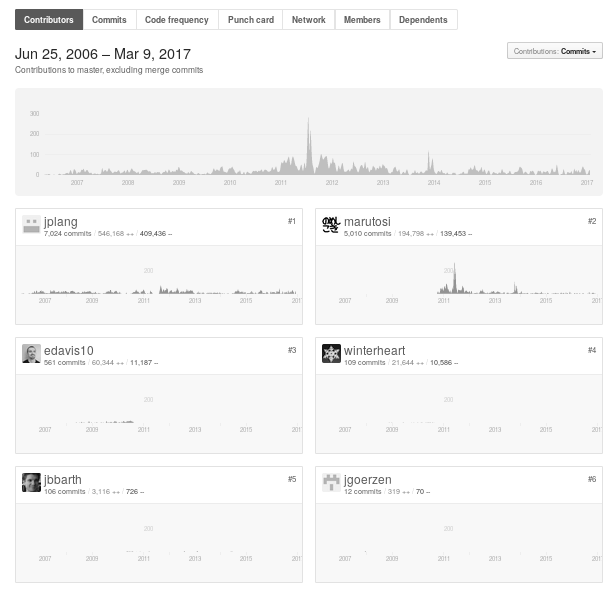
\includegraphics[width=0.8\linewidth]{./chapter-sugestoes-melhorias-fgrm/img/redmine_contribuidores.png}
	\caption{Lista de contribuidores do projeto Redmine}
\label{fig:redmine_contribuidores}
\end{figure}

\subsection{Desenho do Questionário}
\label{ssub:sug_melhoria_desenho_questionario}

A fim de coletar a opinião dos participantes foi utilizado um questionário
eletrônico. O formulário foi desenhado com a premissa de ser respondido em um
prazo curto, de preferência entre 5 e 10 minutos. Neste sentido, as perguntas
foram organizadas em dois grupos principais. As questões do primeiro grupo têm
por objetivo coletar a opinião dos profissionais sobre a relevância da
recomendação proposta e o grau de dificuldade em implementá-la. As perguntas
foram estruturadas de maneira a permitir respostas na forma de uma escala de
Likert em que o respondente deveria fornecer o seu nível de concordância para as
declarações que lhe foram apresentadas. No segundo grupo estamos interessados na
formação dos profissionais. Optamos por definir algumas das questões como não
obrigatórias por entendermos que a impossibilidade ou falta de interesse em
responder determinada pergunta não deveria impedir o participante de enviar os
dados de outras questões respondidas.

\subsection{Processo de Aplicação}
\label{ssub:processo_de_aplicação}

O questionário foi encaminhado à amostra de interesse através de correio
eletrônico. O endereço foi coletado diretamente do projeto hospedado no Github.
Foi desenvolvido um \textit{script} na linguagem Python que permite coletar o
endereço de e-mail e automatizar o processo de envio. As mensagem foram
personalizadas de modo a identificar o nome do usuário e o projeto do Github com
base no template exibido a seguir. O pedido de participação foi enviado para um
total de 121 contribuidores.

% \fbox{\begin{minipage}{\textwidth}
% Dear \{\{real\_name \}\}!

% I’m conducting a research supervised by Rodolfo Resende \@-\@
% homepages.dcc.ufmg.br/~rodolfo and we want to evaluate a collection of
% recommendations to new features in Issue Tracking System. As part of them, we
% planned and executed a survey aiming at to reach a large-scale population of
% practitioners interested in to improve the features of that type of tool. Based
% on your area of interest, we kindly invite you to take part in the following
% survey:

% \{\{url\_formulario\}\}

% You were chosen because your contribution in the project \{\{nome\_grupo\}\}
% \@-\@ \{\{url\_grupo\}\} hosted on the Github platform. Your opinion is
% essential to strength our findings. Please, help us answering this survey until
% May 05th. It takes 05 minutes. As soon as we conclude the data analysis, we will
% share the results with all participants and the software engineering community.
% If you have already fulfilled this questionnaire, please ignore this email.

% Thanks in advance,
% Vagner Clementino.

% \end{minipage}}

O processo de envio consistia ainda de uma segunda mensagem de ``lembrete'' após
dois dias. Esta estratégia foi adotada com base em estudos que discutem os
resultados de que o reenvio pode ser um dos fatores que aumenta a taxa de
participação em levantamentos por questionários realizados através da
web~\cite{fan2010factors}.

\section{Resultados da Avaliação das Sugestões de Melhorias}
\label{sec:resultados_avaliacao_sug_de_melhorias}

Após o envio do formulário aos participantes obtivemos um total de 29 respostas.
Como algumas das questões do formulário não eram de preenchimento obrigatório
algumas perguntas não totalizam 29 respostas. O nível de participação foi
similar ao observado em outros estudo em Engenharia de Software que utilizam o
levantamento por questionário (survey) como método de coleta de
dados~\cite{fan2010factors}. Nas próximas seções apresentamos o perfil dos
participantes, a relevância das sugestões propostas e o grau de facilidade de
implementação das mesmas.

\subsection{Perfil dos Participantes}
\label{sub:sug_melhorias_resultados_perfil_dos_participantes}

No levantamento realizado incluímos uma questão sobre qual sistema o
desenvolvedor contribui. Esta informação é importante porque contribuidores que
trabalham com ferramentas que são consideradas mais famosas e poderosas podem
ter uma maior resistência quanto à inclusão de novas funcionalidades. A
Tabela~\ref{tab:projetos_participantesmy-label} exibe o nome dos projetos que
tiveram contribuidores que preencheram o nosso formulário. Verificamos nas
primeiras posições ferramentas tradicionais como Mantis, Trac e Debbugs. As
FGRMs que tiveram menos de duas participações foram agrupados sob o termo
``OUTROS''.

\begin{table}[htpb]
\centering
\resizebox{.3\textwidth}{!}{%
\begin{tabular}{@{}cc@{}}
\toprule
\textbf{Projeto} & \textbf{Participantes} \\ \midrule
DEBBUGS & 4 \\
MANTISBT & 4 \\
TRAC & 4 \\
FOSSIL & 3 \\
BUGZILLA & 2 \\
REDMINE & 2 \\
OUTROS & 6 \\
\bottomrule
\end{tabular}%
}
\caption{Projetos que os participantes contribuem.}
\label{tab:projetos_participantesmy-label}
\end{table}

Com relação à função desempenhada mais da metade dos participantes são
desenvolvedores (53\%). O segundo grupo de cargo com maior frequência são
aqueles ligados à gerenciamento de equipes (Gerentes de Projetos, Chief
Technical Officer e etc.). Verificamos ainda a participação de Engenheiros e
Arquitetos de Software. Sobre o tempo de experiência, o percentual de 45\% dos
respondentes têm entre dez e vinte anos de experiência. A maior parte desempenha
suas atividades em equipes com 2 a 5 pessoas ou com mais do 10 membros. Quando
questionamos sobre qual o tipo de atividade desempenhada pelo participante,
cerca de 85\% trabalham com desenvolvimento ou manutenção de software. Com base
no perfil apurado entendemos que os participantes são adequados para efetuar a
análise das sugestões de melhorias desta dissertação.

\subsection{Relevância das Sugestões}
\label{sub:sug_melhorias_resultados_relevancia}

As sugestões de melhorias foram apresentadas aos participantes e eles respondiam
se achavam as sugestões pertinentes mediante uma escala de Likert. Os resultados
podem ser visualizados na Figura~\ref{fig:plot_likert_avaliacao_sug_melhorias}.
Em uma primeira análise verificamos que a maioria das recomendações tiveram uma
avaliação positiva dos participantes (Concordo ou Concordo Fortemente). A
exceção foi para a Sugestão \#3 que trata da possibilidade de ordenar as RMs a
serem analisadas pela reputação do Reportador. Por outro lado, as Sugestões \#6
e \#8 tiveram uma boa aceitação dos participantes.

\begin{figure}[htpb]
    \centering
    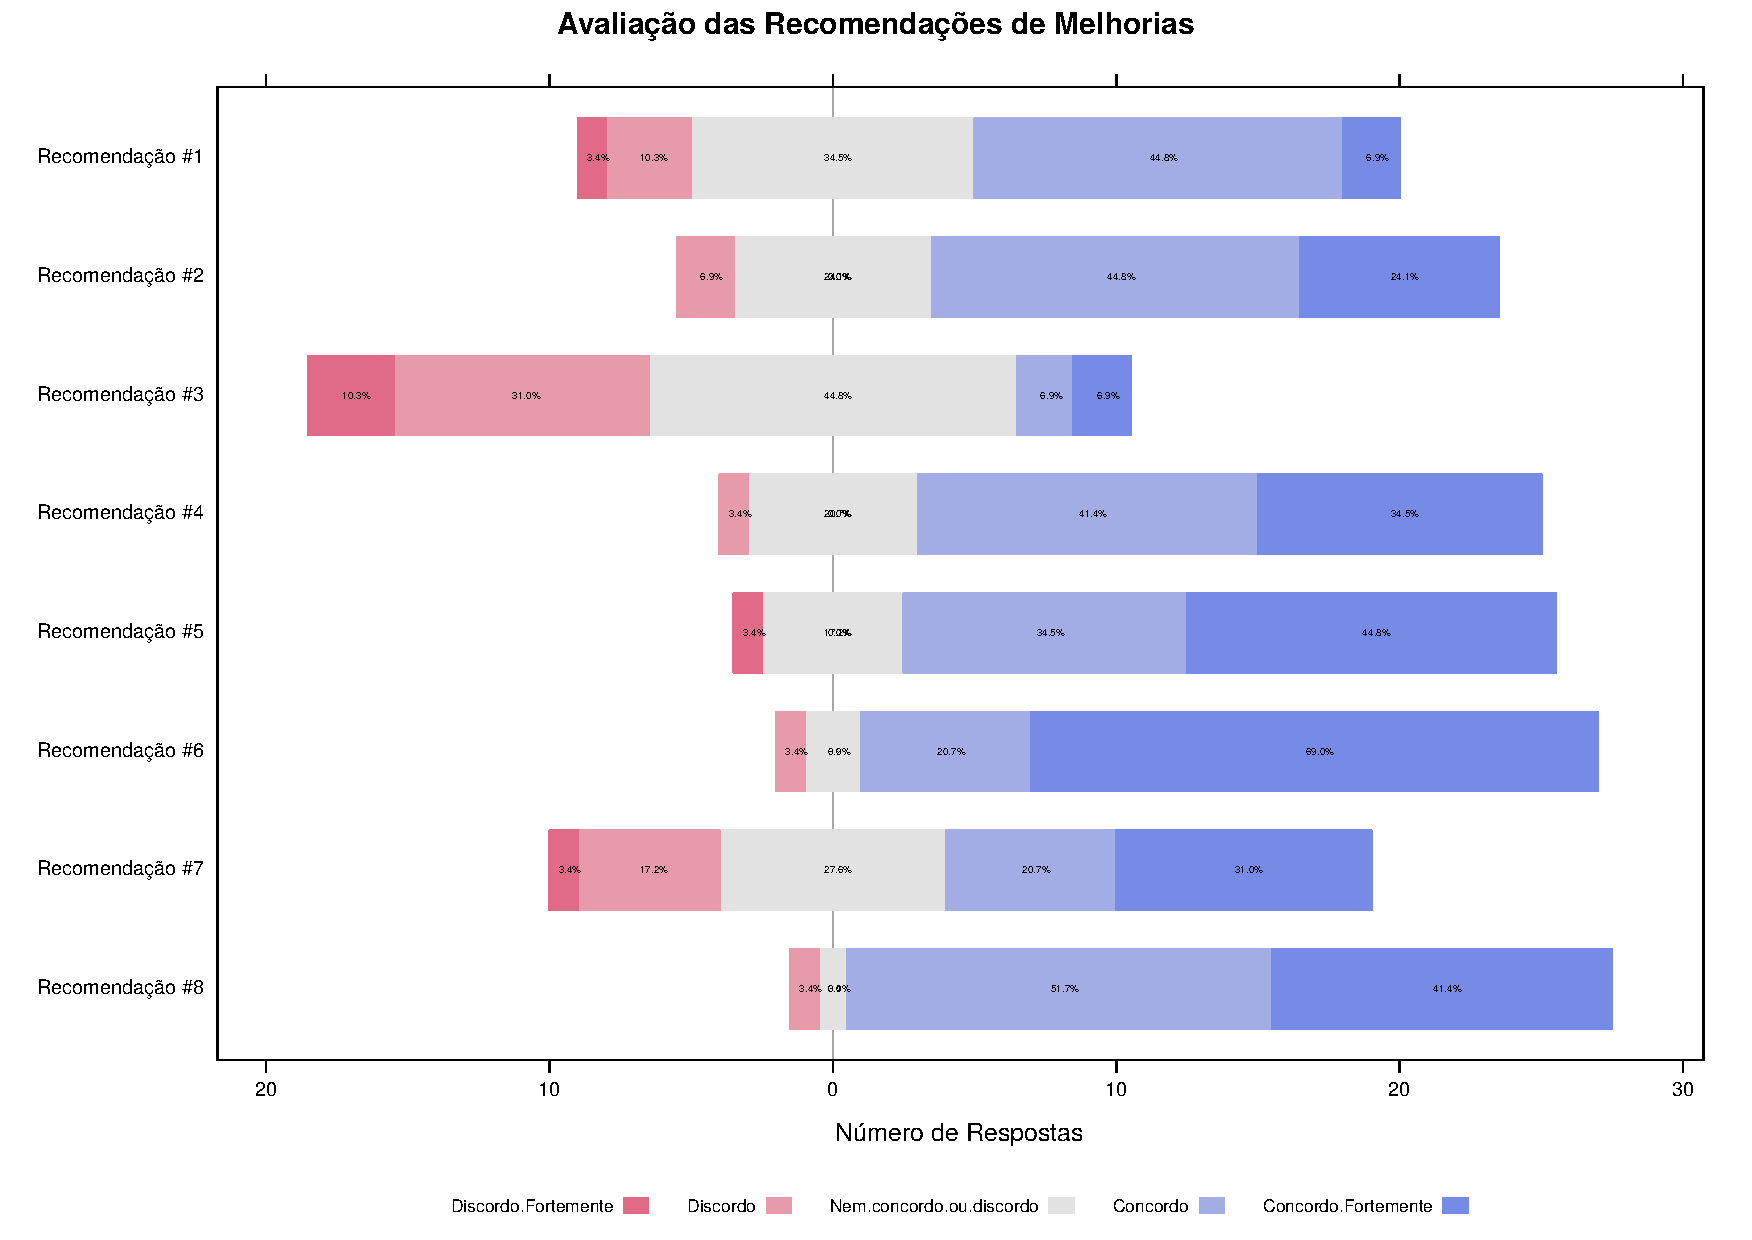
\includegraphics[width=1.1\linewidth]{chapter-sugestoes-melhorias-fgrm/img/plot_likert_avaliacao_sug_melhorias.pdf}
    \caption{Avaliação das Sugestões de Melhorias}
\label{fig:plot_likert_avaliacao_sug_melhorias}
\end{figure}

Para avaliar quais sugestões tiveram maior aceitação definimos um ranqueamento.
O ordenamento consistiu em aplicar pesos para cada item da escala de Likert
conforme a Tabela~\ref{tab:pesos_rank_sug_melhorias}. O valor é obtido
multiplicando a frequência de determinado item da escala pelo seu respectivo
peso. A Tabela~\ref{fig:plot_likert_avaliacao_sug_melhorias} exibe as
recomendações ordenadas pelo nível de aceitação dos participantes. É possível
visualizar o número de respostas que cada item recebeu.

\begin{table}[htpb]
\centering
\resizebox{.3\textwidth}{!}{%
\begin{tabular}{@{}lc@{}}
\toprule
\multicolumn{1}{c}{\textbf{Item da Escala}} & \textbf{Peso} \\ \midrule
Discordo Fortemente & -2 \\
Discordo & -1 \\
Nem concordo ou discordo & 0 \\
Concordo & 1 \\
Concordo Fortemente & 2 \\ \bottomrule
\end{tabular}%
}
\caption{Pesos utilizados para ordenar as sugestões propostas.}
\label{tab:pesos_rank_sug_melhorias}
\end{table}

Com base na Tabela~\ref{tab:ranking-sugestoes-melhorias} verificamos que
recomendações que sobressaíram: utilização nas FGRMs de uma linguagem além do
texto simples para redigir uma RM (\#3), suporte à tarefas colaborativas (\#8) e
incorporação de processos de Integração Contínua (\#5). Por outro lado as
sugestões de diferenciar as RMs pela reputação do Reportador (\#3) e avaliar a
qualidade do relato (\#1) não foram avaliadas como as mais relevantes pelos
participantes. É importar notar que as recomendações que ficaram nas últimas
posições tiveram a opção ``Não concordo nem discordo'' selecionadas com maior
frequência. Este fato pode indicar que não houve uma rejeição pelos
participantes, mas possivelmente, uma baixa compreensão do que estava sendo
proposto.

\begin{table}[htpb]
\centering
\resizebox{\textwidth}{!}{%
\begin{tabular}{@{}lcccccc@{}}
\toprule
\multicolumn{1}{c}{\textbf{Recomendações}} & \textbf{Discordo Fortemente} &
\textbf{Discordo} & \textbf{Não concordo e nem discordo} & \textbf{Concordo} &
\textbf{Concordo Fortemente} & \textbf{Ranking} \\ \midrule
\textit{Sugestão \#6} & 0 & 1 & 2 & 6 & 20 & 45 \\
\textit{Sugestão \#8} & 0 & 1 & 1 & 15 & 12 & 38 \\
\textit{Sugestão \#5} & 1 & 0 & 5 & 10 & 13 & 34 \\
\textit{Sugestão \#4} & 0 & 1 & 6 & 12 & 10 & 31 \\
\textit{Sugestão \#2} & 0 & 2 & 7 & 13 & 7 & 25 \\
\textit{Sugestão \#7} & 1 & 5 & 8 & 6 & 9 & 17 \\
\textit{Sugestão \#1} & 1 & 3 & 10 & 13 & 2 & 12 \\
\textit{Sugestão \#3} & 3 & 9 & 13 & 2 & 2 & -9 \\ \bottomrule
\end{tabular}%
}
\caption{Ranking das sugestões propostas}
\label{tab:ranking-sugestoes-melhorias}
\end{table}

\subsection{Implementação das Sugestões}
\label{sub:sug_melhorias_resultados_implementacao}

Neste etapa do estudo estávamos interessados em avaliar o nível de dificuldade
para implementar as sugestões propostas. Os resultados estão apresentados na
Figura~\ref{fig:plot_likert_avaliacao_implementacao_melhorias}.

\begin{figure}[htpb]
    \centering
    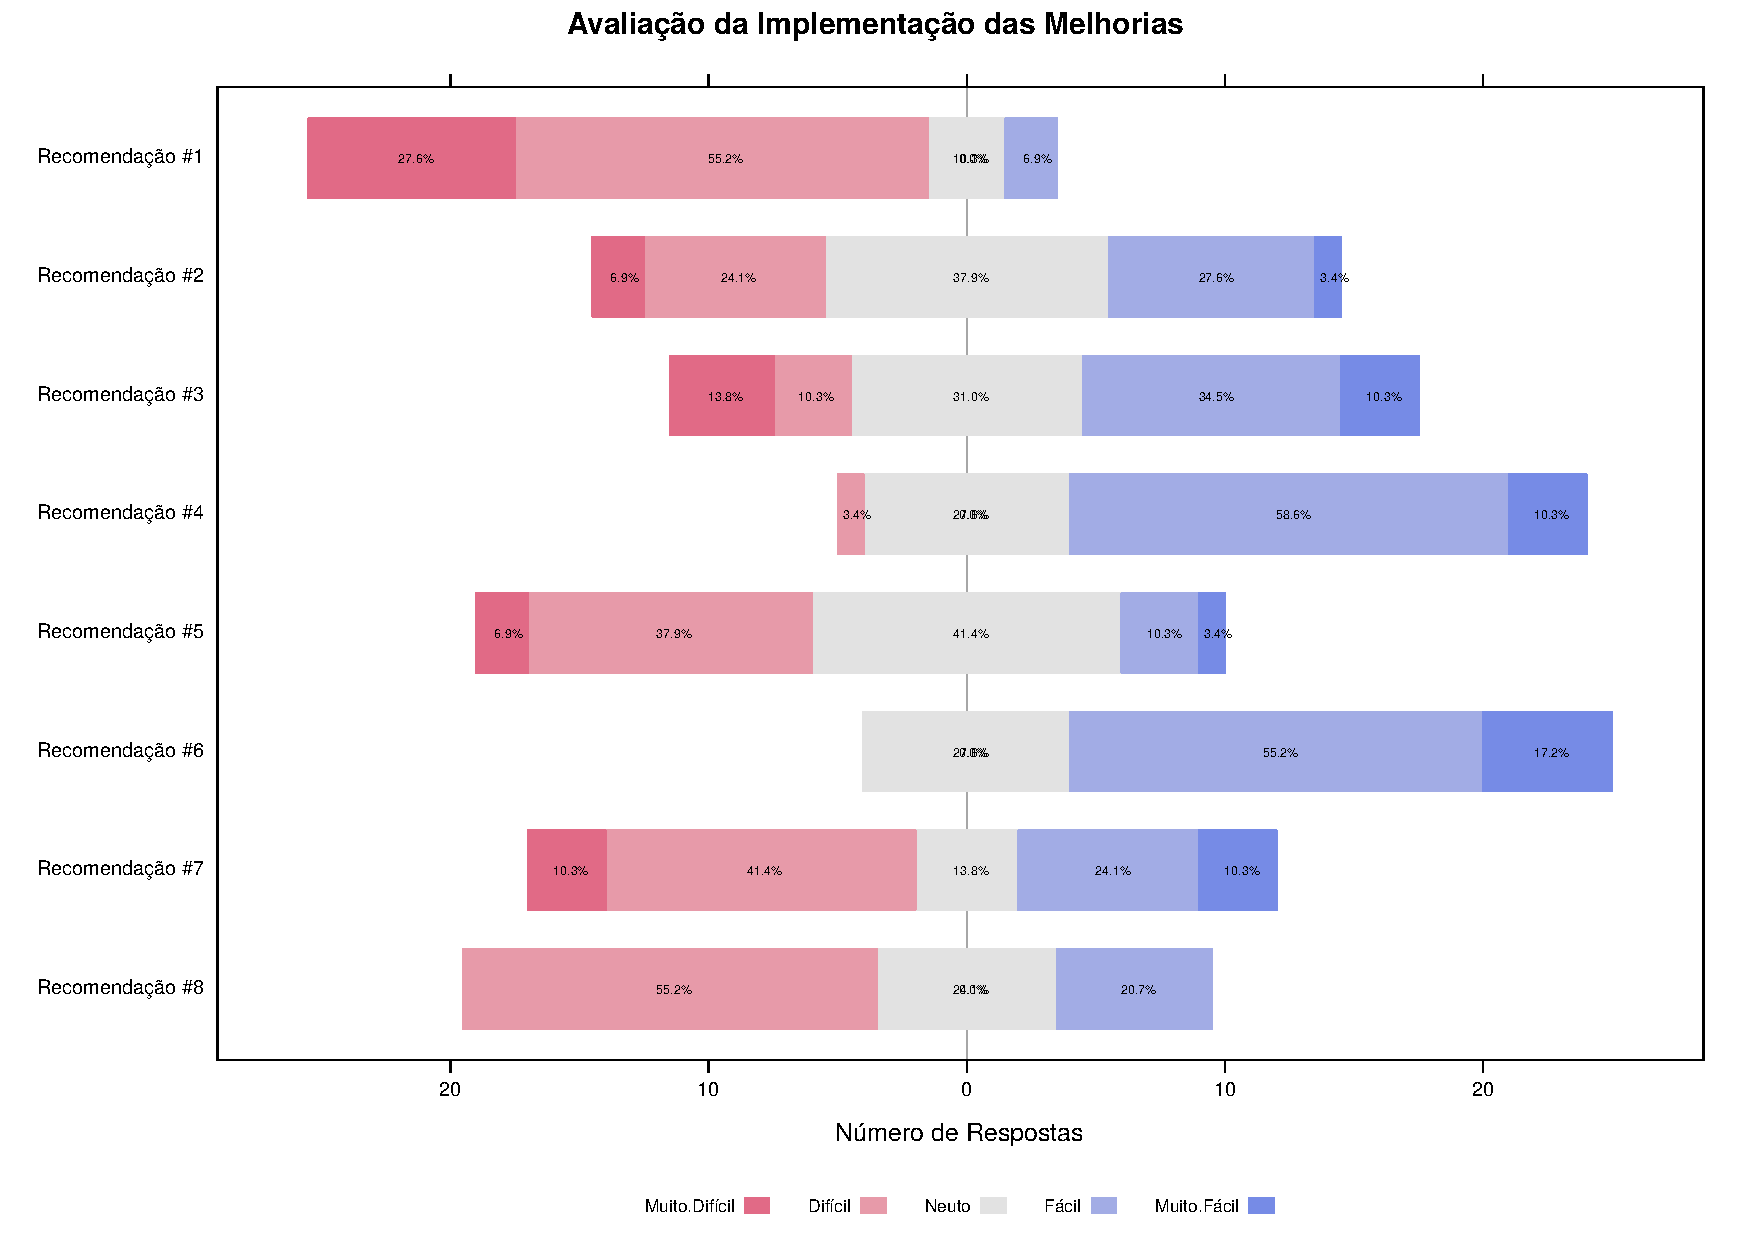
\includegraphics[width=1.1\linewidth]{chapter-sugestoes-melhorias-fgrm/img/plot_likert_avaliacao_implementacao_melhorias.pdf}
    \caption{Avaliação sobre a  implementação das sugestões propostas.}
\label{fig:plot_likert_avaliacao_implementacao_melhorias}
\end{figure}

As sugestões foram ordenadas pelo grau de dificuldade de implementação.
Utilizamos um mecanismo similar ao descrito na
Seção~\ref{sub:sug_melhorias_resultados_relevancia} em que o valor é obtido
multiplicando a frequência de um item da escala por valor previamente definido,
que chamamos de peso. Os pesos estão apresentados na
Tabela~\ref{tab:pesos-implementacao-sug-melhorias}.

\begin{table}[htpb]
\centering
\resizebox{.2\textwidth}{!}{%
\begin{tabular}{@{}ll@{}}
\toprule
Item da Escala & Peso \\ \midrule
Muito Difícil & -2 \\
Difícil & -1 \\
Neutro & 0 \\
Fácil & 1 \\
Muito Fácil & 2 \\ \bottomrule
\end{tabular}%
}
\caption{Pesos utilizados no ranqueamento das sugestões de melhorias}
\label{tab:pesos-implementacao-sug-melhorias}
\end{table}

Foram consideradas ser de fácil implementação: o suporte do relato de uma RM
além do texto simples (\#6), a criação de atalhos e filtros personalizáveis
(\#4) e o ranqueamento das RMs pela reputação do Reportador (\#3). Segundo os
participantes funções como o suporte a tarefas compartilhadas (\#8) e análise da
qualidade do relato (\#1) foram consideradas de um maior grau de dificuldade de
implementação. O fato interessante é que a Sugestão \#3 foi considerada como
uma das mais fáceis de implementar, entretanto, está entre aquelas que tiveram
menor aceite entre os participantes. Este fato pode sugerir que sua possível
rejeição não estaria ligada à sua complexidade de desenvolvimento, mas a fatores
como não haver interesse em classificar aqueles que reportam uma RM\@. Em geral,
ao analisarmos a Figura~\ref{fig:plot_likert_avaliacao_implementacao_melhorias}
é possível verificar que os participantes entenderam que metade das sugestões
propostas possuem uma dificuldade média, enquanto a outra metade pode ser
considerada com um baixo grau de complexidade.

\begin{table}[htpb]
\centering
\resizebox{\textwidth}{!}{%
\begin{tabular}{@{}ccccccc@{}}
\toprule
\multicolumn{1}{l}{\textbf{Recomendações}} & \multicolumn{1}{l}{\textbf{Muito
        Difícil}} & \multicolumn{1}{l}{\textbf{Difícil}} &
\multicolumn{1}{l}{\textbf{Neutro}} & \multicolumn{1}{l}{\textbf{Fácil}} &
\multicolumn{1}{l}{\textbf{Muito Fácil}} & \multicolumn{1}{l}{\textbf{Ranking}}
\\ \midrule
Sugestão \#6 & 0 & 0 & 8 & 16 & 5 & 26 \\
Sugestão \#4 & 0 & 1 & 8 & 17 & 3 & 22 \\
Sugestão \#3 & 4 & 3 & 9 & 10 & 3 & 5 \\
Sugestão \#2 & 2 & 7 & 11 & 8 & 1 & -1 \\
Sugestão \#7 & 3 & 12 & 4 & 7 & 3 & -5 \\
Sugestão \#5 & 2 & 11 & 12 & 3 & 1 & -10 \\
Sugestão \#8 & 0 & 16 & 7 & 6 & 0 & -10 \\
Sugestão \#1 & 8 & 16 & 3 & 2 & 0 & -30 \\
\bottomrule
\end{tabular}%
}
\caption{Ordenamento das sugestões pelo grau de dificuldade.}
\label{tab:ranking_implementacao_sug_melhorias}
\end{table}

\section{Discussão}
\label{sec:sug_melhoria_discussao}

Em geral podemos considerar que as sugestões propostas tiveram uma boa aceitação
dos participantes. Em média 32\% dos participantes avaliaram as recomendações
``Concordo'' ou ``Concordo Fortemente''.  Além disso, por volta de 22\% em média
selecionaram a opção ``Nem concordo ou discordo''. Segundo o nosso entendimento
as respostas poderiam ser alteradas para uma visão mais positiva, com por
exemplo ``Concordo'' ou ``Concordo Fortemente'', caso fossem fornecidos mais
detalhes ao participantes.

Com relação às recomendações propostas, verificamos que a utilização de uma
linguagem além do texto simples, como por exemplo o Markdown, foi muito bem
aceita. Este tipo de sugestão tem como principal objetivo aumentar o poder
de expressão do relato, tal como a possibilidade do destaque da sintaxe do
código fonte. Conforme pode ser observado na
Seção~\ref{sec:caracterizacao_ferramentas} trata-se de uma funcionalidade
encontrada em uma das FGRMs analisadas. Entretanto, o nosso resultado demonstra,
com base na amostra utilizada, que deveria ser estendida para outras
ferramentas.

O suporte à tarefas compartilhadas (sugestão \#8) também foi muito bem aceita.
Esta recomendação surgiu das tentativas de implantação das propostas dos
agilistas~\cite{svensson2005introducing}. A sugestão defende que uma
determinada RM não tenha um único ``dono'', mas que a responsabilidade seja
dividida entre dois ou mais membros da equipe. Esta divisão de tarefas pode
resultar na melhor distribuição do conhecimento entre a equipe. A prevalência
deste tipo de funcionalidade pode estar relacionada com o desejo das equipes de
manutenção de utilizar algumas das práticas dos agilistas. Seria necessário um
aprofundamento da opinião dos participantes para confirmamos esta hipótese.
Apesar da sua popularidade entre os participantes, esta sugestão ficou entre
aquelas com maior grau de dificuldade de implementação.

Por outro lado, as sugestões que têm algum tipo de relação com a interface das
FGRMs (sugestões \#6, \#4, \#3 e \#2) foram consideradas como mais ``fácil'' de
implementar com mais frequência. Entretanto, a sugestão sobre a qualidade do
relato (\#1) ficou entre aquelas com maior grau de dificuldade. Esta
classificação pode ser decorrente do caráter subjetivo que a qualidade do relato
pode ter. Em cada projeto a qualidade do relato pode ter características
distintas o que pode dificultar o seu suporte.

\section{Ameaças à Validade}
\label{sec:sug_melhoria_ameacas}

Para avaliarmos as sugestões propostas utilizamos um levantamento empregando uma
amostra de conveniência. Apesar da taxa de resposta estar dentro da faixa
observada na literatura, o total de participantes não nos permite extrapolar os
resultados para todos os contextos em que as FGRMs estão inseridas.
Adicionalmente, os critérios utilizados para seleção, como por exemplo, seis
meses de desenvolvimento ou ter no mínimo duzentas revisões, não nos permite
afirmar que foram escolhidos os projetos mais representativos para o nosso
público-alvo.

A utilização de apenas projetos públicos hospedados no Github pode ter causado
algum tipo de direcionamento, como por exemplo foco em projetos de código
aberto. Além disso, não há garantidas que os critérios utilizados para seleção,
como por exemplo seis meses de desenvolvimento ou ter no mínimo 200 revisões
(commits), não nos permite afirmar que foram escolhidos escolher os projetos
mais representativos.

A estrutura das perguntas do formulário pode ter causado impacto na quantidade
de respostas ou na opção escolhida pelos participantes. Esta situação pode ter
ocorrido especialmente quando apresentamos as sugestões. No caso de escrevermos
de maneira extensa a explicação corremos o risco do respondente desistir do
item. Entretanto, se o texto fosse escrito de forma ``concisa'' corremos o risco
de ficar vago, o que pode ter impacto nas respostas. A
Tabela~\ref{tab:projetos_participantesmy-label} detalha os projetos que os
participantes contribuem. É possível observar que os participantes trabalham com
ferramentas que são mais famosas e portanto têm o viés de visão mais
``tradicional''.

Em um dos comentários um dos participantes citou que algumas das sugestões
propostas podem ter funcionalidades similares em outras FGRMs. Acreditávamos que
a escolha destas 08 sugestões envolveria as principais características, mas
existe possibilidade de ficar alguma característica relevante de fora.
Infelizmente, posteriormente, julgamos que poderíamos ter incluído mais
sugestões.

\section{Resumo do Capítulo}
\label{sec:sug_melhoria_resumo}

O objetivo do levantamento foi avaliar as sugestões de melhorias de
funcionalidades das FGRMs. A avaliação foi realizada com base na opinião de
desenvolvedores que contribuem para projetos de código aberto deste tipo de
software. Em geral, as sugestões de melhorias foram bem avaliadas. Mais de 30\%
avaliaram as recomendações de forma positiva (``Concordo'' ou  ``Concordo
Fortemente''). Quanto a dificuldade de implementação, metade delas foi
considerada de fácil implementação. No próximo capítulo discutimos aspectos de
implementação da Sugestão \#1 na plataforma Github.
